% !TeX program = pdfLaTeX
\documentclass[12pt]{article}
\usepackage{amsmath}
\usepackage{graphicx,psfrag,epsf}
\usepackage{enumerate}
\usepackage{natbib}
\usepackage{textcomp}
\usepackage[hyphens]{url} % not crucial - just used below for the URL
\usepackage{hyperref}

%\pdfminorversion=4
% NOTE: To produce blinded version, replace "0" with "1" below.
\newcommand{\blind}{0}

% DON'T change margins - should be 1 inch all around.
\addtolength{\oddsidemargin}{-.5in}%
\addtolength{\evensidemargin}{-.5in}%
\addtolength{\textwidth}{1in}%
\addtolength{\textheight}{1.3in}%
\addtolength{\topmargin}{-.8in}%

%% load any required packages here



% tightlist command for lists without linebreak
\providecommand{\tightlist}{%
  \setlength{\itemsep}{0pt}\setlength{\parskip}{0pt}}



\usepackage[dvipsnames]{xcolor} % colors
\newcommand{\ear}[1]{{\textcolor{blue}{#1}}}
\newcommand{\svp}[1]{{\textcolor{RedOrange}{#1}}}
\newcommand{\rh}[1]{{\textcolor{Green}{#1}}}
\usepackage[capitalise]{cleveref}
\newcommand\pcref[1]{(\cref{#1})}
\usepackage{algorithm,algpseudocode,booktabs}

\begin{document}


\def\spacingset#1{\renewcommand{\baselinestretch}%
{#1}\small\normalsize} \spacingset{1}


%%%%%%%%%%%%%%%%%%%%%%%%%%%%%%%%%%%%%%%%%%%%%%%%%%%%%%%%%%%%%%%%%%%%%%%%%%%%%%

\if0\blind
{
  \title{\bf Perception and Cognitive Implications of Logarithmic Scales
for Exponentially Increasing Data: Perceptual Sensitivity Tested with
Statistical Lineups}

  \author{
        Emily A. Robinson 1 \\
    Department of Statistics, California Polytechnic State University -
San Luis Obispo\\
     and \\     Reka Howard 2 \\
    Department of Statistics, University of Nebraska - Lincoln\\
     and \\     Susan VanderPlas 3 \\
    Department of Statistics, University of Nebraska - Lincoln\\
      }
  \maketitle
} \fi

\if1\blind
{
  \bigskip
  \bigskip
  \bigskip
  \begin{center}
    {\LARGE\bf Perception and Cognitive Implications of Logarithmic
Scales for Exponentially Increasing Data: Perceptual Sensitivity Tested
with Statistical Lineups}
  \end{center}
  \medskip
} \fi

\bigskip
\begin{abstract}
Logarithmic transformations are a standard solution to displaying data
that span several magnitudes within a single graph. This paper
investigates the impact of log scales on perceptual sensitivity through
a visual inference experiment using statistical lineups. Our study
evaluated participant's ability to detect differences between
exponentially increasing data, characterized by varying levels of
curvature, using both linear and logarithmic scales. Participants were
presented with a series of plots and asked to identify the panel that
appeared most different from the others. Due to the choice of scale
altering the contextual appearance of the data, the results revealed
slight perceptual advantages for both scales depending on the curvatures
of the compared data. This study serves as the initial part of a
three-paper series dedicated to understanding the perceptual and
cognitive implications of using logarithmic scales for visualizing
exponentially increasing data. These studies serve as an example of
multi-modal graphical testing, examining different levels of engagement
and interaction with graphics to establish nuanced and specific
guidelines for graphical design.
\end{abstract}

\noindent%
{\it Keywords:} log scales, visual inference, graphical testing
\vfill

\newpage
\spacingset{1.45} % DON'T change the spacing!

\hypertarget{introduction}{%
\section{Introduction}\label{introduction}}

Effective communication of data is critical in influencing people's
opinions and actions. This consideration was particularly true during
the COVID-19 pandemic, where data visualizations and dashboards were
vital in informing the public and policymakers about the outbreak's
status. Local governments relied on graphics to inform their decisions
about shutdowns and mask mandates, while residents were presented with
data visualizations to encourage compliance with these regulations. A
major issue designers encountered when creating COVID-19 plots was how
to display data from a wide range of values
\citep{fagen-ulmschneider_2020, burnmurdoch_2020}. When faced with data
that span several orders of magnitude, we must decide whether to show
the data on its original scale (compressing the smaller magnitudes into
a relatively small area) or to transform the scale and alter the
contextual appearance of the data. Log axis transformations have emerged
as a standard solution to this challenge, as they allow for the display
of data over several orders of magnitude within a single graph.

Exponential data is one such example of a function that compresses
smaller magnitudes into a smaller area; \cref{fig:log-scales} presents
hard drive capacity over the past forty years on both the linear and log
scales to demonstrate the usefulness of log scales when dealing with
data spanning multiple magnitudes. Logarithms facilitate the conversion
of multiplicative relationships (displaying 1 \& 10 with a distance of
10 units apart and displaying 10 \& 100 with a distance of 90 units
apart) to additive relationships (displaying 1 \& 10 and 10 \& 100 an
equal distance apart), highlighting proportional relationships and
linearizing power functions \citep{menge_logarithmic_2018}. Logarithms
also have practical applications, simplifying the computation of small
numbers such as likelihoods and transforming data to conform to
statistical assumptions. Although log scales have a long history of use
in fields such as ecology, psychophysics, engineering, and physics
\citep{heckler_student_2013, waddell2005comparisons}, there is still a
need to understand the implications of their use and provide best
practices for their implementation.

\begin{figure}[tbp]

{\centering 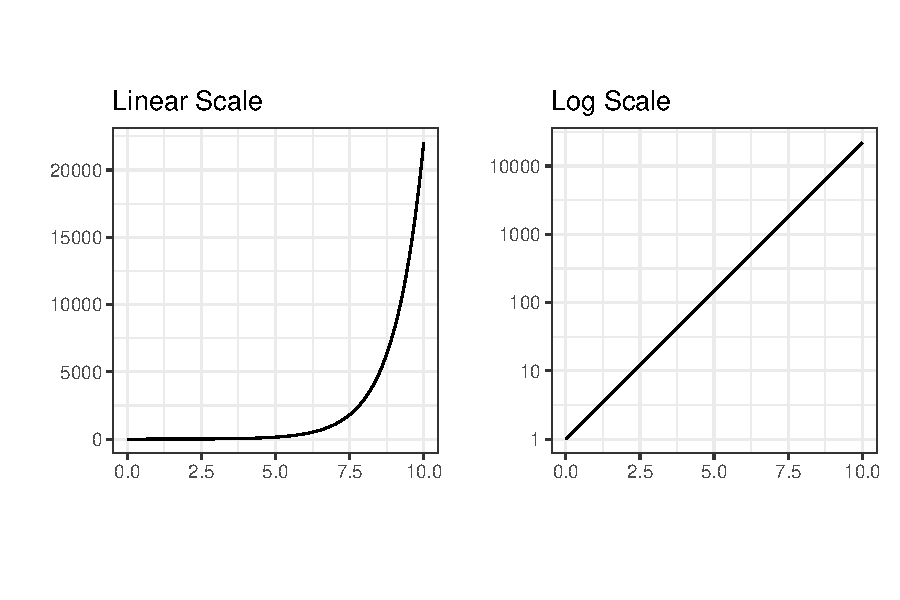
\includegraphics[width=1\linewidth,]{logarithmic-lineups_files/figure-latex/log-scales-1} 

}

\caption[Linear scale versus log scale]{These plots present hard drive capacity over the past forty years on both the linear and log scale and illustrate the use of the log scale when displaying data which spans several magnitudes.}\label{fig:log-scales}
\end{figure}

Apart from the biases resulting from using log scales, there is a
general misinterpretation of exponential growth. Early stages of
exponential growth often appear to have a small growth rate, while the
middle stage seems to exhibit more quadratic growth. It is only in the
later stages that the exponential growth becomes apparent.
\cref{fig:exponential-stages} highlights the three stages and associated
appearances of exponential growth at each stage
\citep{vonbergmann_2021}. This misinterpretation can lead to decisions
made under inaccurate understanding, resulting in potential
consequences.

\begin{figure}[tbp]

{\centering 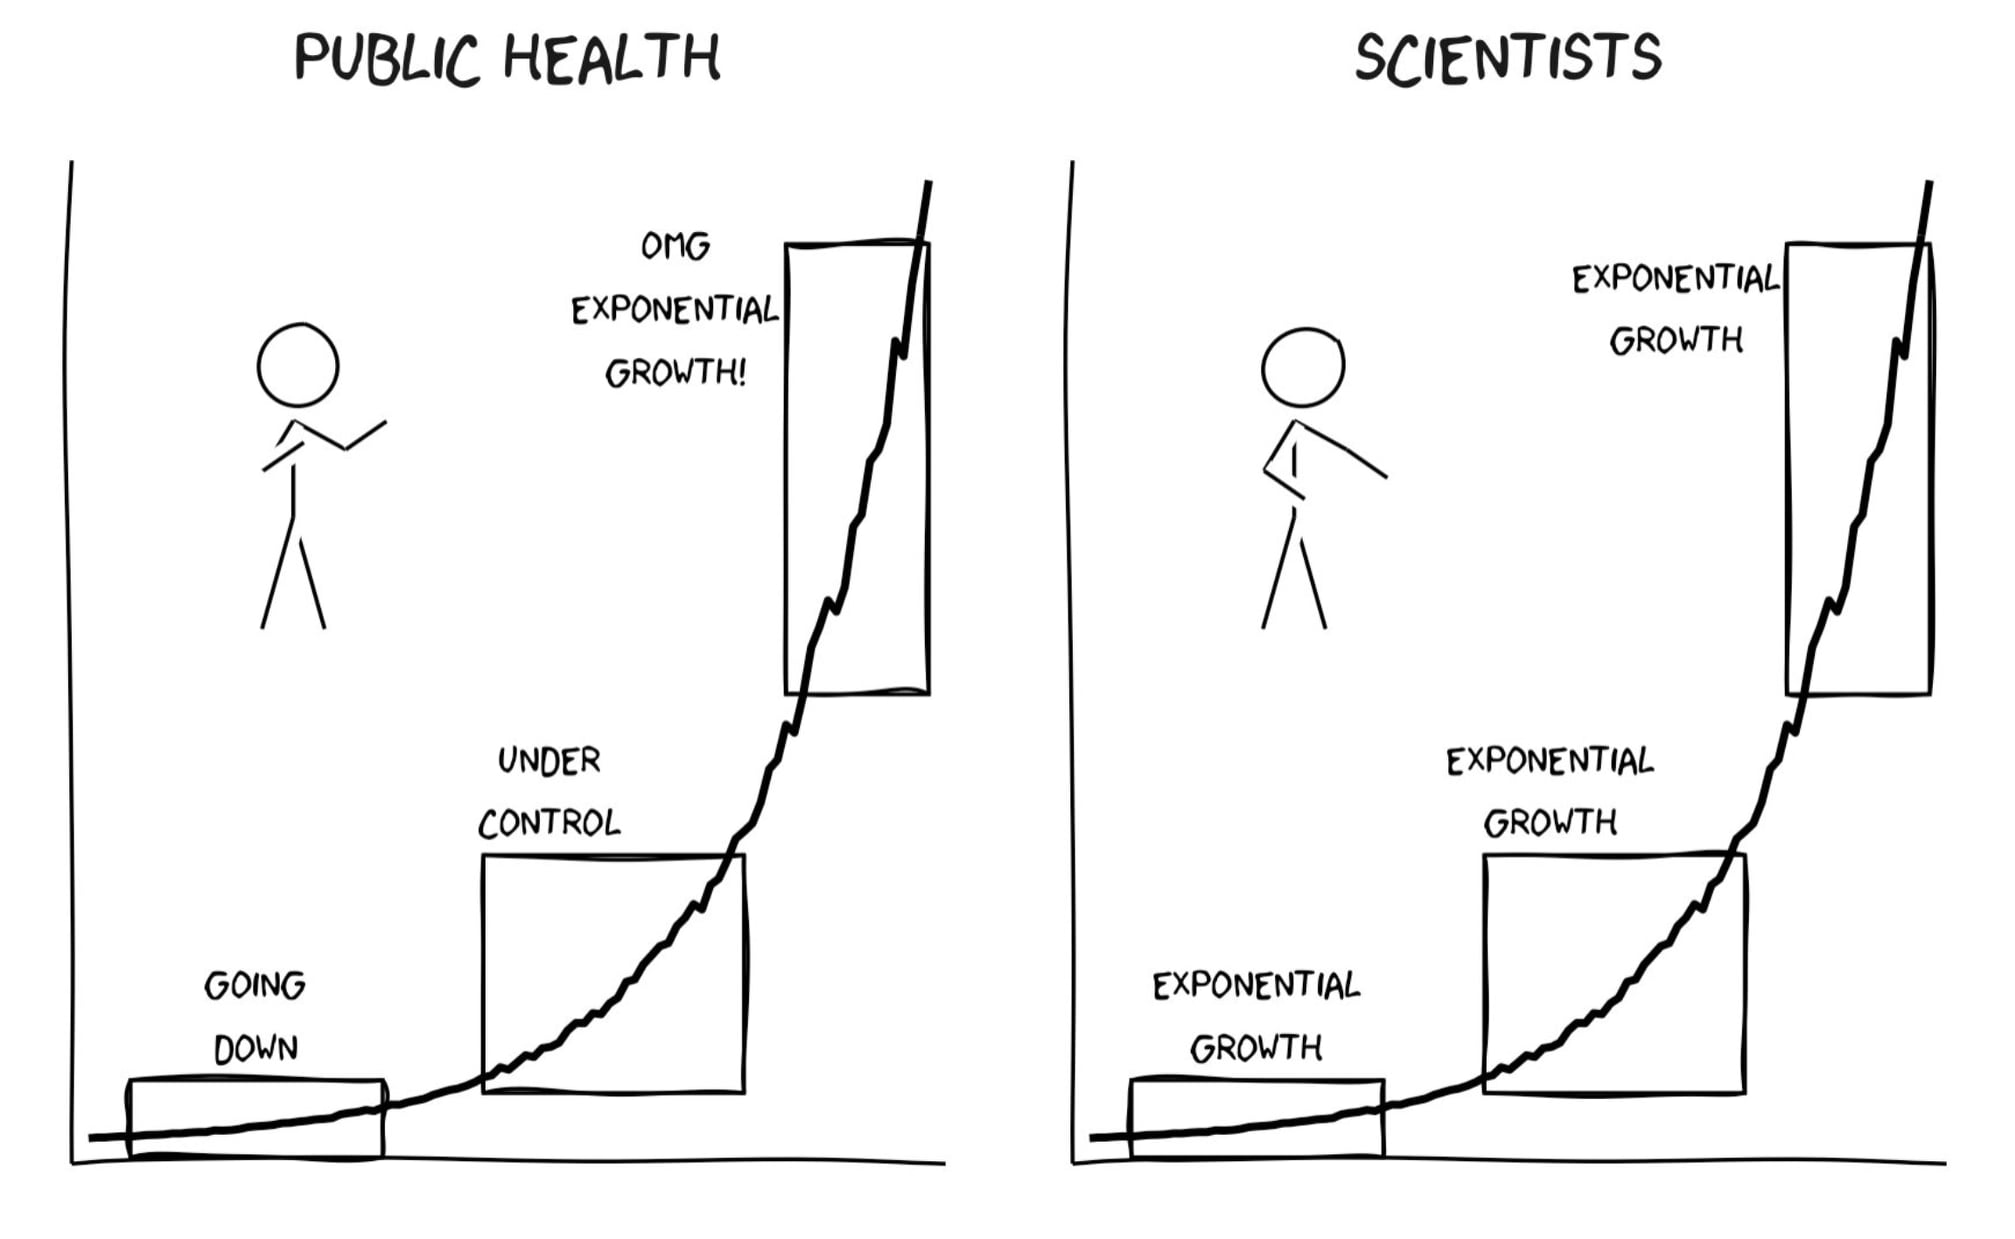
\includegraphics[width=1\linewidth,]{images/exponential-stages-comic} 

}

\caption{This figure highlights the three stages and associated appearances of exponential growth at each stage. Early stages of exponential growth often appear to have a small growth rate, while the middle stage seems to exhibit more quadratic growth. It is only in the later stages that the exponential growth becomes apparent.}\label{fig:exponential-stages}
\end{figure}

Previous studies have explored the estimation and prediction of
exponential growth and found that individuals often underestimate
exponential growth when presented values numerically and graphically
\citep{wagenaar_misperception_1975}. The hierarchy of plot objects, such
as lengths and angles, as described by \citet{cleveland_graphical_1985},
offers a possible explanation for the underestimation observed in
exponentially increasing trends. Experiments conducted by
\citet{wagenaar_misperception_1975}, \citet{jones_polynomial_1977}, and
\citet{mackinnon_feedback_1991} aimed to improve estimation accuracy for
exponential growth. While contextual knowledge or experience did not
enhance estimation, instruction on exponential growth reduced
underestimation by prompting participants to adjust their initial
starting value
\citep{wagenaar_misperception_1975, jones_polynomial_1977}. Furthermore,
providing immediate feedback to participants about the accuracy of their
predictions improved estimation \citep{mackinnon_feedback_1991}.

Log transforming the data may address our inability to predict
exponential growth accurately. However, this transformation introduces
new complexities, as most readers may need to be mathematically
sophisticated enough to intuitively understand logarithmic math and
translate it back into real-world effects.
\citet{menge_logarithmic_2018} surveyed ecologists to determine their
encounter frequency and comprehension of log-scaled data in the
literature. The authors identified misconceptions encountered when
presented with data on log-log scales which arise from linear
extrapolation assumptions in log-log space, neglecting the underlying
exponential relationship in linear-linear space.

In this paper, we evaluated the benefits and drawbacks of using log
scales and examine their impact on perceptual sensitivity by conducting
a visual inference experiment using statistical lineups
\citep{buja_statistical_2009}. The experiment focused on a participant's
ability to identify differences between exponentially increasing curves
with varying levels of curvature using both linear and log scales. The
study did not require participants receive any mathematical training or
have prior understanding of exponential growth or logarithmic scales,
focusing instead on the fundamental nature of the ability to identify
differences in charts.

\citet{buja_statistical_2009} introduced statistical lineups as a
framework for statistical inference and graphical tests. Statistical
lineups treat a data plot as a visual statistic, summarizing the data as
a numerical function or mapping. Evaluation of a panel in a statistical
lineup requires visual inspection by a person, and if visual evaluations
lead to different results, two visualization methods are deemed
significantly different. Recent studies have utilized statistical
lineups to quantify the perception of graphical design choices
\citep{hofmann_graphical_2012, loy_model_2017, loy_variations_2016, vanderplas_clusters_2017}.
Statistical lineups provide an elegant way of combining perception and
statistical hypothesis testing through graphical experiments
\citep{majumder_validation_2013, vanderplas_testing_2020, wickham2010graphical}.

The term `lineup' is an analogy to police lineups in criminal
investigations, where witnesses identify the criminal from a group of
individuals. Similarly, researchers present a statistical lineup plot
consisting of smaller panels and ask the viewer to identify the panel
that contains the actual data from a set of decoy null plots.
Researchers generate null plots containing data generated according to a
prespecified hypothesis using permutation or simulation. Typically, a
statistical lineup consists of 20 panels, with one target panel and 19
null panels. If the viewer can identify the target panel from the null
panels, it suggests that the actual data is visually distinct from the
data generated under the null model. \cref{fig:lineup-example} presents
examples of statistical lineups. The statistical lineup on the left
presents increasing exponential data displayed on a linear scale with
panel \((5 \times 2) + 3\) as the target. The lineup on the right shows
increasing exponential data plotted on a log scale with panel
\(2 \times 2\) as the target.

While explicit graphical tests direct the participant to a specific
feature of a plot to answer a particular question, implicit graphical
tests require the user to identify both the purpose and function of the
plot in order to evaluate the plots shown. Furthermore, implicit
graphical tests, such as lineups, simultaneously test for multiple
visual features, including outliers, clusters, and linear and nonlinear
relationships \citep{vanderplas2015spatial}. Researchers can collect
responses from multiple viewers using crowd-sourcing websites such as
Prolific and Amazon Mechanical Turk.

\begin{figure}[tbp]

{\centering 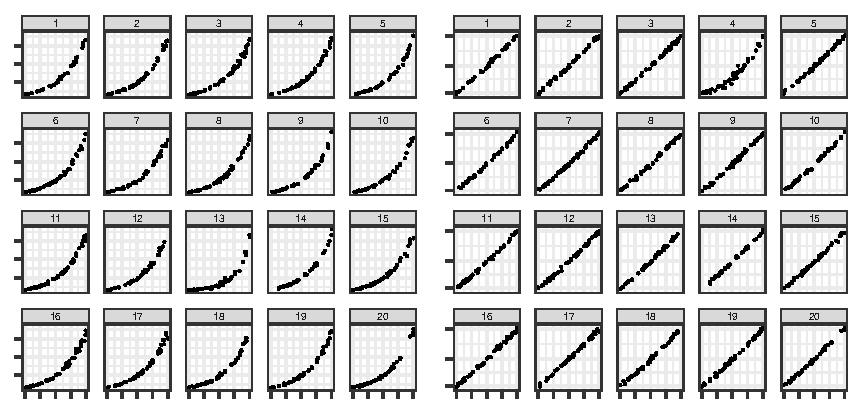
\includegraphics[width=\linewidth,]{logarithmic-lineups_files/figure-latex/lineup-example-1} 

}

\caption[Lineup examples]{The lineup plot on the left displays increasing exponential data on a linear scale with panel (2 x 5) + 3 as the target. The lineup plot on the right displays increasing exponential data on the log scale with panel 2 x 2 as the target.}\label{fig:lineup-example}
\end{figure}

In \protect\hyperlink{methods}{Section 2} we describe the participant
sample, the graphical task, data generation process, and study design.
\protect\hyperlink{results}{Section 3} describes the participant data
collected and shares results from the statistical analyses of the data
using a generalized linear mixed model. We present overall conclusions
and discussion of the results in
\protect\hyperlink{conclusion-discussion}{Section 4}, and provide an
overview of future related papers. The
\protect\hyperlink{supplementary-material}{Supplementary Material}
includes a link to the RShiny data collection applet, participant data
used for analysis, and code to replicate the analysis. The results of
this study lay the groundwork for further exploration of the
implications of using log scales in data visualization.

\hypertarget{methods}{%
\section{Study Development and Methods}\label{methods}}

\hypertarget{data-generation}{%
\subsection{Data Generation}\label{data-generation}}

In this study, we simulated data from an exponential model to generate
the target and null data sets; the models between panels differ in the
parameter values selected for the null and target panels. In order to
guarantee the simulated data spans the same domain and range of values
for each statistical lineup panel, we began with a domain constraint of
\(x\in [0,20]\) and a range constraint of \(y\in [10,100]\) with
\(N = 50\) points randomly assigned throughout the domain. We mapped the
randomly generated \(x\) values to a corresponding \(y\) value based on
an exponential model with predetermined parameter values and
multiplicative random errors to simulate the response. These constraints
assure that participants who select the target panel are doing so
because of their visual perception differentiating between curvature or
growth rate rather than different starting or ending values.

We simulated data based on a three-parameter exponential model with
multiplicative errors: \begin{align}
y_i & = \alpha\cdot e^{\beta\cdot x_i + \epsilon_i} + \theta \\
\text{with } \epsilon_i & \sim N(0, \sigma^2). \nonumber
\end{align} The parameters \(\alpha\) and \(\theta\) were adjusted based
on \(\beta\) and \(\sigma^2\) to guarantee the range and domain
constraints are met. The model generated \(N = 50\) points
\((x_i, y_i), i = 1,...,N\) where \(x\) and \(y\) have an increasing
exponential relationship. The heuristic data generation procedure is
described in \cref{alg:lineup-parameter-estimation-algorithm} and
\cref{alg:lineup-exponential-data-simulation-algorithm}.

\begin{algorithm}
  \caption{Lineup Parameter Estimation}\label{alg:lineup-parameter-estimation-algorithm}
  \begin{algorithmic}[1]
    \Statex \hspace*{-1em}\textbullet~\textbf{Input Parameters:} domain $x\in[0,20]$, range $y\in[10,100]$, midpoint $x_{mid}$.
    \Statex \hspace*{-1em}\textbullet~\textbf{Output Parameters:} estimated model parameters $\hat\alpha, \hat\beta, \hat\theta$.
    \State Determine the $y=-x$ line scaled to fit the assigned domain and range.
    \State Map the values $x_{mid} - 0.1$ and $x_{mid} + 0.1$ to the $y=-x$ line for two additional points.
    \State From the set of points $(x_k, y_k)$ for $k = 1,2,3,4$, calculate the coefficients from the linear regression model $\ln(y_k) = b_0 +b_1x_k$ to obtain starting values for $\alpha_0 = e^{b_0}, \beta_0 =  b_1, \theta_0 = 0.5\cdot \min(y)$
    \State Using the \texttt{nls} function from the base \texttt{stats} package in Rstudio [@Rstudio] and the starting parameter values - $\alpha_0, \beta_0, \theta_0$ - fit the nonlinear model, $y_k = \alpha\cdot e^{\beta\cdot x_k}+\theta$ to get estimated parameter values for $\hat\alpha, \hat\beta, \hat\theta.$
  \end{algorithmic}
\end{algorithm}

\begin{algorithm}
  \caption{Lineup Exponential Data Simulation}\label{alg:lineup-exponential-data-simulation-algorithm}
  \begin{algorithmic}[1]
    \Statex \hspace*{-1em}\textbullet~\textbf{Input Parameters:} sample size $N = 50$, estimated parameters $\hat\alpha$, $\hat\beta$, and $\hat\theta$, from \cref{alg:lineup-parameter-estimation-algorithm}, and standard deviation $\sigma$ from the exponential curve.
    \Statex \hspace*{-1em}\textbullet~\textbf{Output Parameters:} $N$ points, in the form of vectors $\mathbf{x}$ and $\mathbf{y}$.
    \State Generate $\tilde x_j, j = 1,..., \frac{3}{4}N$ as a sequence of evenly spaced points in $[0,20]$. This ensures the full domain of $x$ is used, fulfilling the constraints of spanning the same domain and range for each parameter combination.
    \State Obtain $\tilde x_i, i = 1,...,N$ by sampling $N = 50$ values from the set of $\tilde x_j$ values. This guarantees some variability and potential clustering in the exponential growth curve disrupting the perception due to continuity of points.
    \State Obtain the final $x_i$ values by jittering $\tilde x_i$.
    \State Calculate $\tilde\alpha = \frac{\hat\alpha}{e^{\sigma^2/2}}.$ This ensures that the range of simulated values for different standard deviation parameters has an equal expected value for a given rate of change due to the non-constant variance across the domain.
    \State Generate $y_i = \tilde\alpha\cdot e^{\hat\beta x_i + e_i}+\hat\theta$ where $e_i\sim N(0,\sigma^2).$
  \end{algorithmic}
\end{algorithm}

\hypertarget{lineups-parameter-selection}{%
\subsection{Parameter Selection}\label{lineups-parameter-selection}}

We chose three levels of trend curvature (low curvature, medium
curvature, and high curvature). For each curvature level, we simulated
1,000 data sets of \((x_{ij}, y_{ij})\) points for \(i = 1,...,50\)
increments of \(x\)-values and replicated \(j = 1,...,10\) corresponding
\(y\)-values per \(x\)-value. Each generated \(x_i\) point from
\cref{alg:lineup-exponential-data-simulation-algorithm} was replicated
ten times. We fit a linear regression model on each of the individual
data sets and computed the lack of fit statistic (LOF) which measures
the deviation of the data from the linear regression model. After
obtaining the LOF statistic for each level of curvature, we evaluated
the density plots (\cref{fig:lof-density-curves}) to provide a metric
for differentiating between the curvature levels and thus detecting the
target plot. While the LOF statistic provides a numerical value for
discriminating between the difficulty levels, it cannot be directly
related to the perceptual discriminability; it serves primarily as an
approximation to ensure that we are testing parameters at several
distinct curvature levels. \cref{tab:parameter-data} lists the final
parameters used for data simulation.

\begin{figure}[tbp]

{\centering 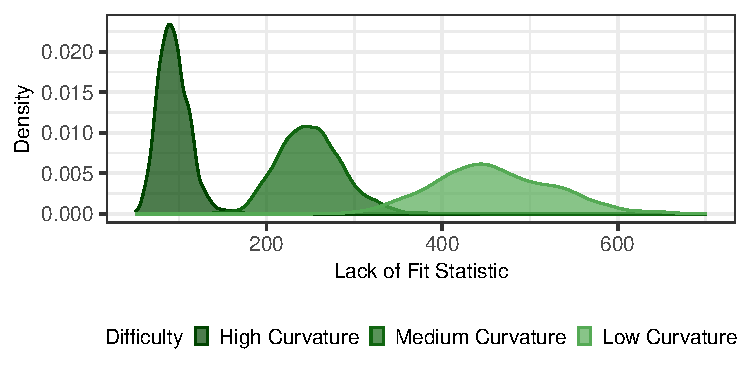
\includegraphics[width=1\linewidth,]{logarithmic-lineups_files/figure-latex/lof-density-curves-1} 

}

\caption[Lineup parameter selection]{Density plot of the lack of fit statistic showing separation of difficulty levels: obvious curvature, noticable curvature, and almost linear.}\label{fig:lof-density-curves}
\end{figure}

\begin{table}

\caption{\label{tab:parameter-data}Lineup data simulation final parameters}
\centering
\begin{tabular}[t]{lrrrrrr}
\toprule
Curvature Level & $x_{mid}$ & $\hat\alpha$ & $\tilde\alpha$ & $\hat\beta$ & $\hat\theta$ & $\hat\sigma$\\
\midrule
High & 14.5 & 0.91 & 0.88 & 0.23 & 9.10 & 0.25\\
Medium & 13.0 & 6.86 & 6.82 & 0.13 & 3.14 & 0.12\\
Low & 11.5 & 37.26 & 37.22 & 0.06 & -27.26 & 0.05\\
\bottomrule
\end{tabular}
\end{table}

\hypertarget{lineup-setup}{%
\subsection{Lineup Setup}\label{lineup-setup}}

To generate the small multiple scatter plots for the statistical lineups
shown to participants in the study, we simulated a single data set
corresponding to curvature level A for the target plot and multiple data
sets corresponding to curvature level B for the null plots. The
\texttt{nullabor} package in R \citep{buja_statistical_2009} randomly
assigned the target plot to one of the panels surrounded by panels
containing null plots. For example, the statistical lineup randomly
embeds a target plot with simulated data following an increasing
exponential curve with high curvature within null plots with simulated
data following an increasing exponential trend with low curvature. The
target and null panels spanned a similar domain and range due to the
implemented constraints when simulating the data. There were a total of
six lineup curvature combinations;
\cref{fig:curvature-combination-example} illustrates the six lineup
curvature combinations (top: linear scale; bottom: log scale) where the
green solid line indicates the curvature level designated to the target
plot while the black dashed line indicates the curvature level assigned
to the null plots. Two sets of each lineup curvature combination were
simulated (a total of twelve test data sets) and plotted on both the
linear scale and the log scale (24 test lineup plots). In addition,
three curvature combinations generated homogeneous ``Rorschach''
lineups, where all panels were from the same distribution. Each
participant evaluated one ``Rorschach'' lineup, but for simplicity, we
did not describe these evaluations, and we left their analysis to a
later date.

\begin{figure}[tbp]

{\centering 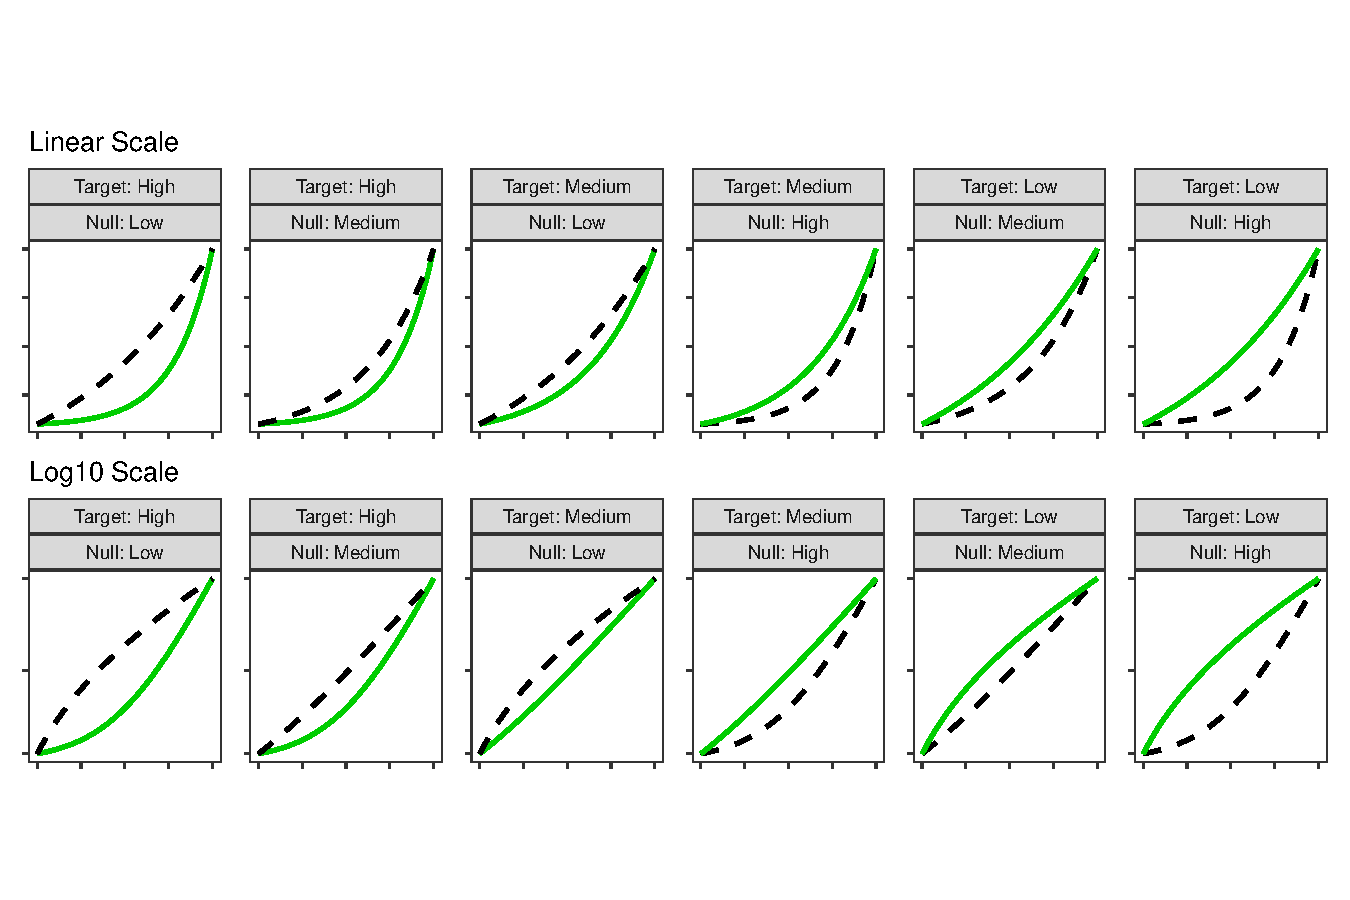
\includegraphics[width=1\linewidth,]{logarithmic-lineups_files/figure-latex/curvature-combination-example-1} 

}

\caption[Lineup curvature combinations]{Thumbnail plots illustrating the six curvature combinations displayed on both scales (linear and log). The green solid line indicates the curvature level to be identified as the target plot from amongst a set of null plots with the curvature level indicated by the black dashed line.}\label{fig:curvature-combination-example}
\end{figure}

\hypertarget{study-design-and-implementation}{%
\subsection{Study Design and
Implementation}\label{study-design-and-implementation}}

We used Prolific, a survey site that connects researchers to study
participants, to recruit participants above the age of majority in their
region; we did not request a representative sample, previous literature
suggests there are minor effects of demographics on the outcome of
graphical experiments involving lineups
\citep{vanderplas2015spatial, majumder_validation_2013}. Following the
completion of the current statistical lineup study, participants
sequentially completed two additional graphical experiments related to
the perception of logarithmic scales (to be discussed at a later date),
and we compensated them for their participation in the series of all
three studies.

We showed each participant 13 lineup plots (12 test and one Rorschach).
At the start of the study, we randomly assigned participants to one of
the two replicate data sets for each of the six unique lineup curvature
combinations. Participants evaluated the lineup plot corresponding to
the linear and log scales for each assigned test data set. For the
additional Rorschach lineup plot, we randomly assigned participants to
one data set shown on either the linear or the log scale. We randomized
the order in which participants saw the assigned 13 lineup plots.

\cref{fig:study-homepage} presents a screenshot of the study homepage,
which served as an introduction to participants and guided them through
the series of three graphical experiments. The first experiment,
discussed in this paper, utilized statistical lineups to investigate the
effect of logarithmic scales on perceptual sensitivity. The second
experiment, incorporated an interactive `You Draw It' feature introduced
by \citet{aisch2015you} and employed in the study by
\citet{robinson2022eye}, to examine the effect of logarithmic scales on
prediction. The third experiment focused on numerical estimation and
cognitive understanding of logarithmic scales.

Participants completed the series of graphical tests using an R Shiny
application \citep{shiny_pkg} accessible at
\url{https://emily-robinson.shinyapps.io/perception-of-statistical-graphics-log/}.
The code used to create the study application is available on GitHub at
\url{https://github.com/earobinson95/perception-of-statistical-graphics-log}.
Before completing the lineup study, the `You Draw It' study, and the
estimation study, participants were prompted to provide their
demographic information. The series of studies received an IRB exemption
(IRB \#20200720178EX) from the University of Nebraska - Lincoln.

\begin{figure}[tbp]

{\centering 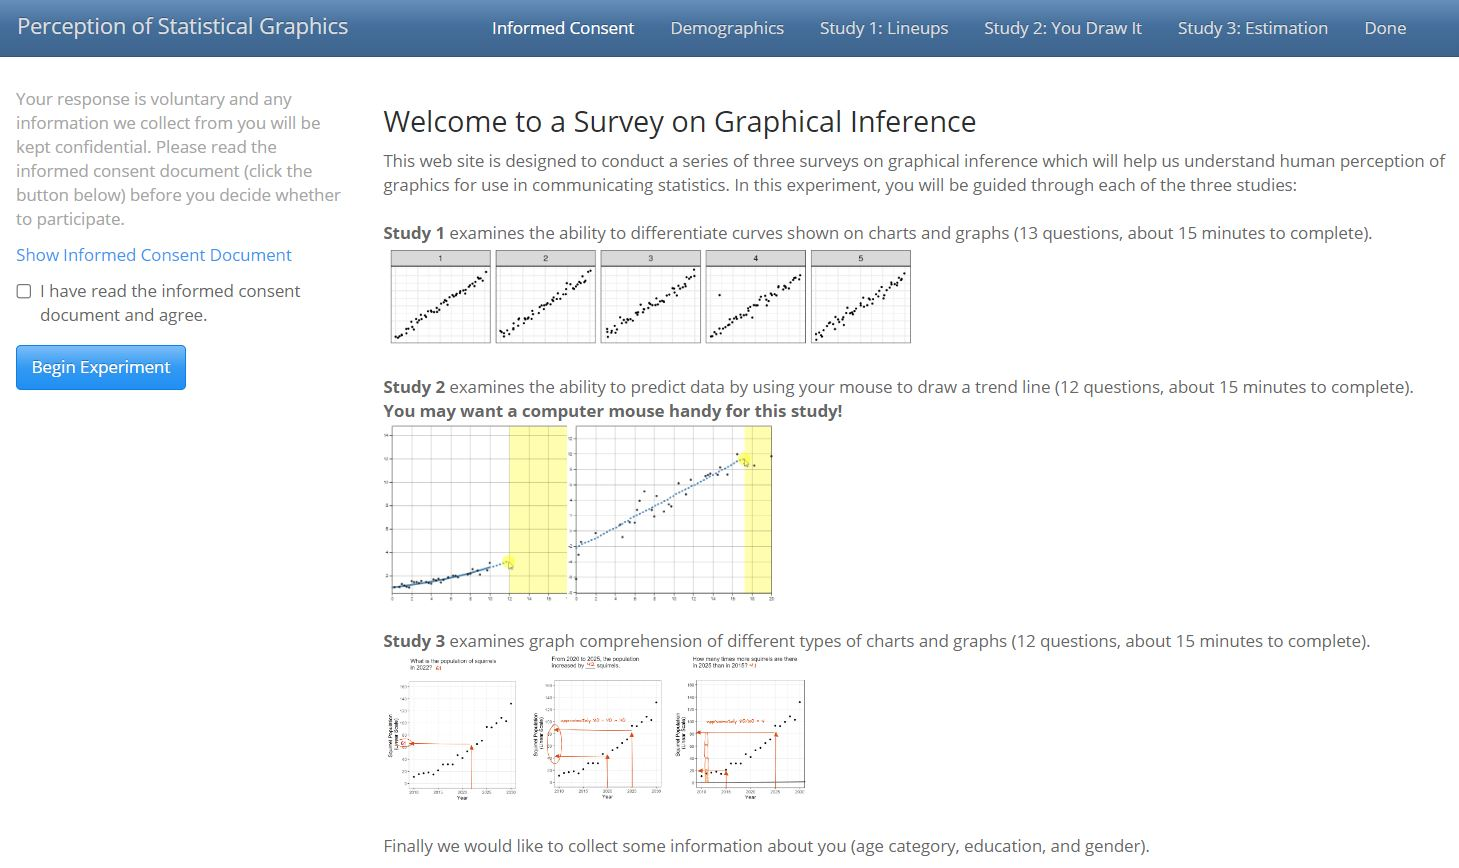
\includegraphics[width=1\linewidth,]{images/study-homepage} 

}

\caption[Study applet homepage]{Screenshot of the study applet homepage guiding participants through the series of three graphical experiments related to the perception of logarithmic scales.}\label{fig:study-homepage}
\end{figure}

The statistical linenup study guided participants through the series of
13 lineup plots and asked them to identify the plot which appeared to be
most different from the others (\cref{fig:lineup-study-example-trial}).
In each lineup evaluation, participants justified their choice and
provided their level of confidence in their choice. This graphical task
aimed to test an individual's ability to perceptually differentiate
exponentially increasing trends with differing levels of curvature on
both the linear and log scales.

\begin{figure}[tbp]

{\centering 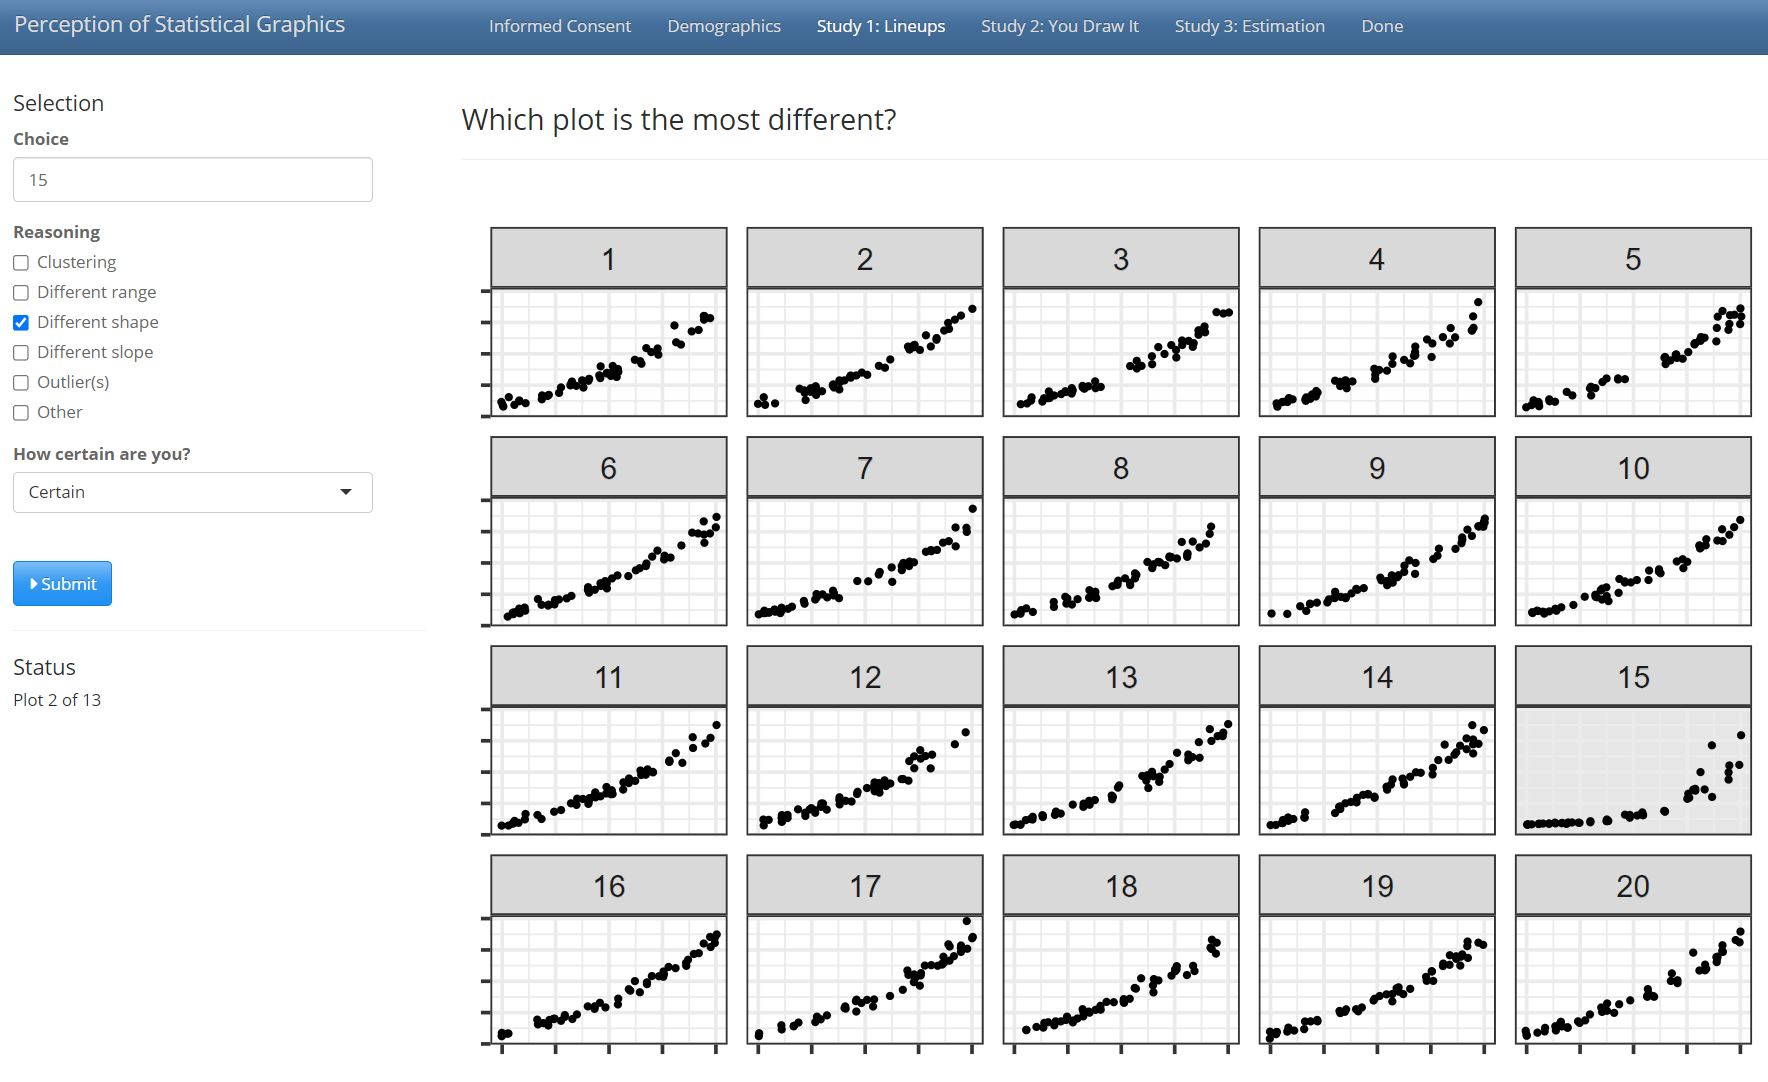
\includegraphics[width=1\linewidth,]{images/lineup-study-example-trial} 

}

\caption[Lineup study example trial]{Screenshot of an example trial participants see when completing the lineup study. The applet guided participants through 13 lineup plots and asked them to identify the plot which appeared to be the most different from the others.}\label{fig:lineup-study-example-trial}
\end{figure}

\hypertarget{statistical-analysis}{%
\subsection{Statistical Analysis}\label{statistical-analysis}}

Each lineup plot evaluated was assigned a binary value based on the
participant response (correct target plot identification = 1, not
correct target plot identification = 0). We defined \(Y_{ijkl}\) as the
event that participant \(l = 1,...,N_\text{participant}\) correctly
identified the target plot for data set \(k = 1,2\) with curvature
combination \(j = 1,2,3,4,5,6\) plotted on scale \(i = 1,2\). The binary
response was analyzed using a generalized linear mixed model (GLMM)
following a binomial distribution with a logit link function with a
row-column blocking design accounting for the variation due to
participant and data set, respectively, as \begin{equation}
\text{logit }P(Y_{ijk}) = \eta + \delta_i + \gamma_j + (\delta \gamma)_{ij} + s_l + d_k
\end{equation} \noindent where

\begin{itemize}
\item $\eta$ is the baseline average probability of selecting the target plot
\item $\delta_i$ is the effect of scale $i = 1,2$
\item $\gamma_j$ is the effect of curvature combination $j = 1,2,3,4,5,6$
\item $(\delta\gamma)_{ij}$ is the two-way interaction between the $i^{th}$ scale and $j^{th}$ curvature combination
\item $s_l \sim N(0,\sigma^2_\text{participant})$ is the random effect for participant characteristics
\item $d_k \sim N(0,\sigma^2_{\text{data}})$ is the random effect for data specific characteristics. 
\end{itemize}

\noindent We assumed the random effects for data set and participant are
independent. Target plot identification was analyzed using a GLMM
implemented in \texttt{glmer} from the \texttt{lme4} R (version 4.2.2)
package \citep{lme4}. We used the \texttt{emmeans} R package
\citep{emmeans} to calculate the estimated target detection
probabilities and obtain odds ratio comparisons between the log and
linear scale.

\hypertarget{results}{%
\section{Results}\label{results}}

We recruited participants and conducted the study via Prolific, a
crowd-sourcing website, in March 2022. The study included a diverse
group of participants, with an inner-quartile age range between 23 and
31 and a median age of 26 years old. Among the participants, 59\%
self-identified as male, 40\% as female, and 1\% as
variant/nonconforming. Additionally, individuals from more than 21
countries participated in the study and 97\% of the participants
indicated fluency in English. Moreover, 81\% of the participants
reported having completed some undergraduate courses or higher. During
data collection, 325 individuals completed 4,492 individual test lineup
evaluations. We included only participants in the final analysis who
completed the entire study, which included 311 participants and 3,958
lineup evaluations. Due to server capacity, some participants were
required to restart the study, thus resulting in the possibility of more
than twelve lineup evaluations per participant. As a whole, participants
evaluated each uniquely generated lineup plot between 141 and 203 times
(Mean: 164.92, SD: 14.9). Participants correctly identified the target
panel in 47\% of the 1,981 lineup evaluations made on the linear scale
and 65.3\% of the 1,977 lineup evaluations made on the log scale.

The results from the GLMM indicated a strong interaction between the
curvature combination and scale (\(\chi^2_5 = 294.443\);
\(\text{p} <0.0001\)), and the estimated variance due to participant and
data set were \(\hat\sigma^2_{\text{participant}} = 1.19\) (s.e. = 1.09)
and \(\hat\sigma^2_{\text{data}} = 0.433\) (s.e. = 0.66), respectively.
Therefore, we concluded that there was low variability in the accuracy
of target panel detection between participants and across replications
of uniquely simulated data sets. To determine the effect of scale, we
compared the estimated accuracy between the log and linear scale within
each curvature combination due to the interaction as determined by the
GLMM.

On both the log and linear scales, the highest accuracy occurred in
lineup plots where the target model and null model had a considerable
difference in curvature, and the target plot had more curvature than the
null plots (high curvature target plot embedded in low curvature null
plots). There was a decrease in accuracy on the linear scale when
comparing a target plot with less curvature to null plots with more
curvature (medium curvature target plot embedded in high curvature null
plots; low curvature target plot embedded in medium curvature null
plots; low curvature target plot embedded in high curvature null plots).
\citet{best_perception_2007} found that the accuracy of identifying the
correct curve type was higher when presented with nonlinear trends,
indicating that it is hard to say something is linear (i.e., something
has less curvature), but easy to say that it is not linear; our results
concur with this observation. \cref{fig:odds-ratio-plot} displays the
estimated (log) odds ratio of successfully identifying the target panel
on the log scale compared to the linear scale. The thumbnail figures to
the right of the plot illustrate the curvature combination on the linear
(left thumbnail) and log base ten (right thumbnail) scales associated
with the \(y\)-axis label. The choice of scale had no impact if the
curvature differences were substantial and the target plot had more
curvature than the null plots (high curvature target plot embedded in
low curvature null plots). However, presenting data on the log scale
makes us more sensitive to slight changes in curvature (low or high
curvature target plot embedded in medium curvature null plots; medium
curvature target plot embedded in high curvature null plots) and
apparent differences in curvature when the target plot had less
curvature than the null plots (low curvature target plot embedded in
high curvature null plots). An exception occurred when identifying a
plot with curvature embedded in null plots close to a linear trend
(medium curvature target panel embedded in low curvature null panels).
The results indicate that participants were more accurate at detecting
the target panel on the linear scale than on the log scale. When
examining this curvature combination, the same perceptual effect
occurred as we previously saw, but in a different context of scales. On
the linear scale, participants were perceptually identifying a convexly
curved trend from close to a linear trend, whereas after the logarithmic
transformation, participants were perceptually identifying a trend close
to linear from a concavely curved trend
(\cref{fig:curvature-combination-example}). This result again supports
the claim that it is easy to identify a curve in a group of lines but
harder to identify a line in a group of curves
\citep{best_perception_2007}.

\begin{figure}[tbp]

{\centering 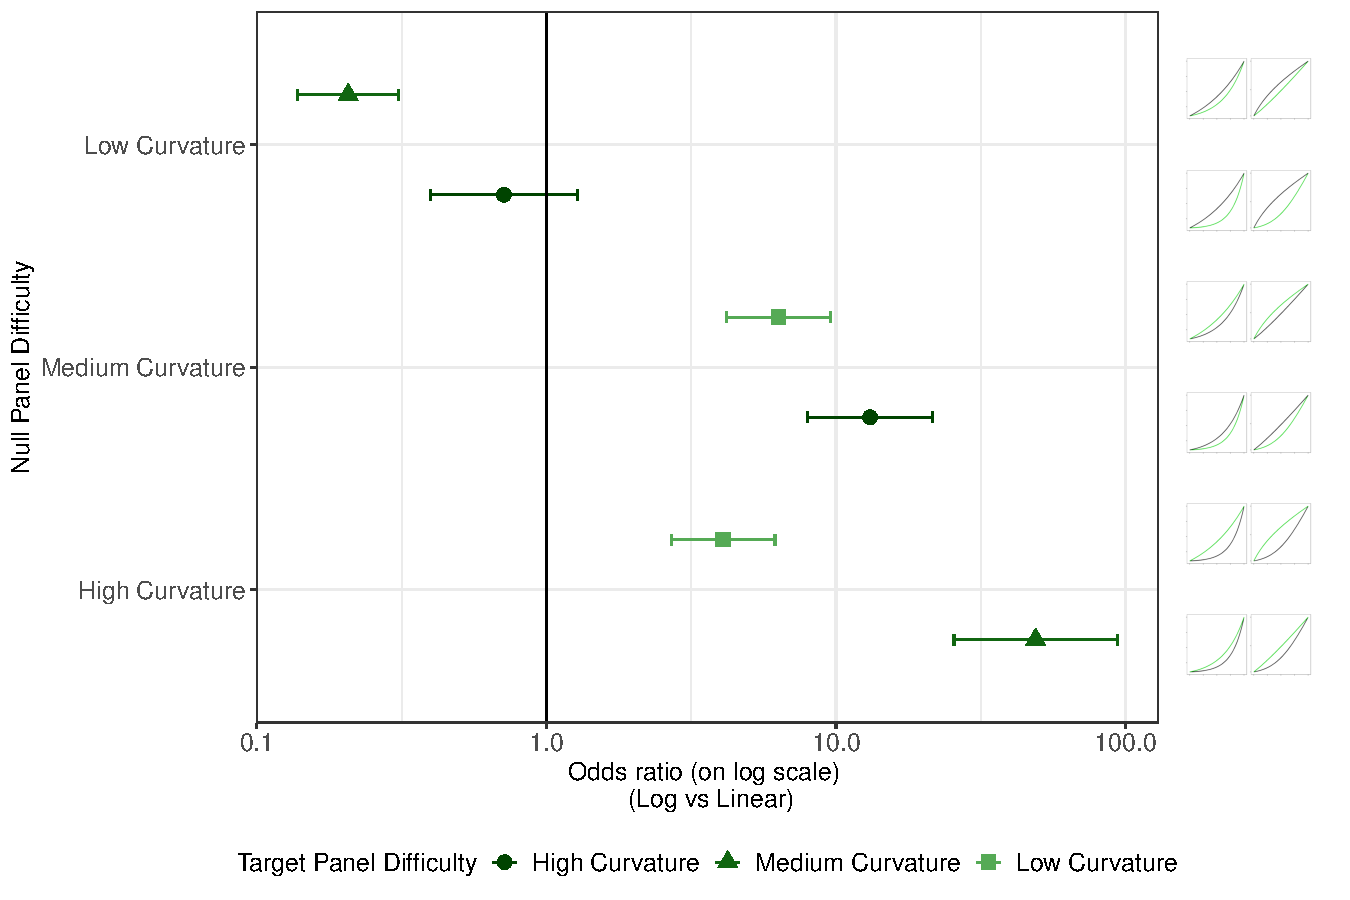
\includegraphics[width=\linewidth,]{logarithmic-lineups_files/figure-latex/odds-ratio-plot-1} 

}

\caption[Lineups log(odds) results]{Estimated (log) odds ratio of successfully identifying the target panel on the log scale compared to the linear scale. The y-axis indicates the the model parameters used to simulate the null plots with the target plot model parameter selection designated by shape and shade of green. The thumbnail figures on the right display the curvature combination as shown in \cref{fig:curvature-combination-example} on both scales (linear - left, log - right).}\label{fig:odds-ratio-plot}
\end{figure}

\hypertarget{discussion-conclusion}{%
\section{Discussion and Conclusion}\label{discussion-conclusion}}

This work aims to provide foundational research to support the
principles that guide design decisions in scientific visualizations of
exponential data. In this study, we explored the use of linear and log
scales to determine whether the choice of scale impacts our ability to
notice differences in exponentially increasing trends. The results
indicated that when there was a considerable difference in curvature
between the target plot and null plots and the target plot had more
curvature than the null plots, the choice of scale had no impact, and
participants accurately differentiated between the two curves on both
the linear and log scale. However, displaying exponentially increasing
data on a log scale improved the accuracy of differentiating between
models with slight curvature differences or apparent curvature
differences when the target plot had less curvature than the null plots.
An exception occurred when identifying a plot with curvature embedded in
surrounding plots perceived close to a linear trend, indicating that it
is easy to identify a curve in a group of lines but much harder to
identify a line in a group of curves. Using visual inference to identify
these guidelines suggests that there are perceptual advantages to log
scales when differences are subtle.

We conducted this study as the first in a series of three graphical
tests to understand the perceptual and cognitive implications of using
log scales to display exponentially increasing data. In our next two
papers in this series, we will investigate whether using log scales
presents cognitive disadvantages, such as making it harder to utilize
graphical information. These studies serve as an example of multi-modal
graphical testing, examining different levels of engagement and
interaction with graphics in order to produce nuanced, specific
guidelines for graphical design. By testing graphics in situations
similar to how they are used in practice, we can gain additional insight
into graphical perception and improve visual communication of scientific
results.

\hypertarget{supplementary-material}{%
\section*{Supplementary Material}\label{supplementary-material}}
\addcontentsline{toc}{section}{Supplementary Material}

\begin{itemize}
\tightlist
\item
  \textbf{Participant Data:} De-identified participant data collected in
  the study and used for analyses (lineup-model-data.csv).
\item
  \textbf{Data Analysis Code:} The code used to replicate the analysis
  in this paper (lineups-analysis.qmd).
\item
  \textbf{Study Applet Code:} The code used to create the study applet
  via RShiny can be found on GitHub at
  \url{https://github.com/earobinson95/perception-of-statistical-graphics-log}
\item
  \textbf{README:} File containing detailed descriptions of the
  supplementary material. (README.html).
\end{itemize}

\bibliographystyle{agsm}
\bibliography{bibliography.bib}


\end{document}
